\documentclass[../main.tex]{subfiles}
\begin{document}
\chapter{Results}
\label{chap:resconc}

\section{Results and Caveats}

Many difficulties connected with this research result from the fact that almost all the documents produced by the \textbf{RTCA}, the \textbf{EUROCAE} and the \textbf{ICAO} are expensive commercial products and each of them ranges between 300 and 500 dollars. Therefore every piece of necessary information had to be acquired in an alternative way: either by conferences slides, papers or articles.

Regarding \textit{dump1090} the extracted binaries behave differently from what was expected: the one from FlightRadar24 does not visually output any information on the screen but it is modified to upload data directly inside their network. On the other hand the binary extracted from the Stratux image have a strange behavior since, if fed with the \textit{1090\_small.bin} data file and given the \textit{-{}-no-crc-check} option it correctly outputs messages with CRC errors while the version from the \textit{Antirez} repository, which is supposed to be the same as the extracted one, using the same file and parameters does not show such messages.

Working with the Unicorn Engine was neither easy nor straightforward. This emulator is really powerful and well developed; however, it comes with no documentation at all but just a couple of C or Python basic examples. Therefore, every time that more details were needed it was necessary to take a look at the source code and understand how to use a specific function or how a feature was implemented. Moreover, even if Unicorn is capable of emulating the ARM architecture in almost all his functionalities, it does not have default support for Vector Floating Point (VFP) instructions, which are widely used in the tested binary. Although this behavior, according to the ARM processor documentation, is the correct one, it resulted in the emulator not being able to recognize VFP instructions. As a consequence the template crashes while in execution. Following the ARM documentation and the issues in the Unicorn Engine repository it was possible to create a piece of Assembly code to enable VFP as in Figure \ref{fig:vfp} and \ref{fig:vfp1}.

\begin{figure}[htp]
  \centering
  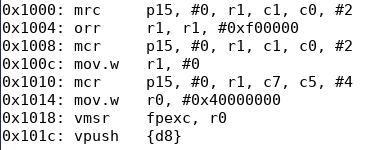
\includegraphics[scale=0.9]{images/vfpdisass.png}
  \caption{Assembly code to enable VFP instructions}
  \label{fig:vfp}
\end{figure}
\begin{figure}[htp]
  \centering
  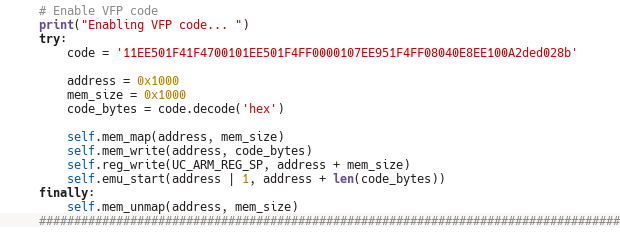
\includegraphics[scale=0.9]{images/vfpcode.png}
  \caption{Portion of python code to enable VFP instructions}
  \label{fig:vfp1}
\end{figure}

Even after the emulator was able to run VFP instructions a lot of debugging was needed to make a single template work, as it is quite common to have illegal memory access also in relation to library functions such as \textit{puts, printf, etc} that need to be properly handled.

The Unicorn Engine has also a strange behavior when run on the multicore server. A quick investigation was carried out to understand more and the same template was run on different systems and different Operating Systems. In particular on two laptops, of which one was running Arch Linux 64bit with Linux Kernel 4.15.2 and the other one running Ubuntu Linux 16.04 LTS 32bit, the Unicorn Engine has exactly the same behavior on both Laptops.

The same behavior was also tested on a virtual machine running Fedora 27 64-bit while the same template run on the multicore server gives completely different results in terms of final register state. With the insertion of some debug lines inside the template it was possible to understand that on the server the emulation reaches immediately the end of the function, while the normal behavior observed in the other cases, establishes that the emulation should cycle inside the function. It is still unclear why the emulator has this behavior only on the server. It might depend on some problems regarding the size of the RAM or on the fact that it is a shared machine and the operating system runs inside a container or virtualized environment.

In addition to this, \textit{afl-unicorn} was developed as an internal research project in a cybersecurity company. Although it is a great tool there is little to no documentation on his functioning and more importantly there is no real walkthrough on how to properly create a template for a binary. This is not a real problem since everything is clearly explained in the blog post about \textit{afl-unicorn} and in the basic template provided. However, having to "work your way" through the tool is a great way to understand how it works but it requires quite a lot of time.

\textbf{AFL} had problems in finding crashes on the analyzed software and, in some cases, even in the intentionally vulnerable binaries. This can be caused by many factors:

\begin{enumerate}

  \item The used test input was not good enough, therefore, it will require a great deal of time for \textbf{AFL} to generate an input capable of triggering the vulnerability. This is also supported by the extremely low and slow growing code coverage obtained during the tests.

  \item The vulnerability was actually triggered but the overflow did not cause any crashes, therefore resulting in a corrupted zombie program that might
  never crash. Moreover, \textbf{AFL} cannot detect memory leaks and other types of corruption in the target even though those are very likely security bugs.
  This type of problem is quite common in embedded devices as it has been widely detailed and analyzed in~\cite{corrcrash}.

  \item It is possible that the code being tested is written with security in   mind and therefore no bugs are present in the code. The original author of
  \textit{dump1090}, Salvatore Sanfilippo\footnote{\url{http://invece.org/}}, has a strong security background and this might have influenced the security of code. However, the programs that have been tested are not the ones used in the real embedded systems in airplanes, which can have even worse implementations of the protocols.

  \item Even if \textbf{AFL} represents the current state of the art in terms of binary fuzzing it might not be the proper tool to use in this situation.

\end{enumerate}

As already mentioned acquiring data for \textit{dump978} was a trivial process since it is not used in Europe. Moreover, \textit{extract\_nexrad} does not implement any functions to use Huffman encoding which was the most promising part since it is likely to be vulnerable. The sample \textbf{FIS-B} (text and image) data acquired from the GDL90 document~\cite{gdl90} are not correctly decoded both by \textit{extract\_nexrad} and by \textit{uat2text}. Further investigation discovered that there have been at least 2 revisions of the \textbf{RTCA} documents, such as RTCA DO-267A, that introduced changes in APDUs and packet formats. Some of those modifications, that are adopted in Europe under particular documents: \acrlong{etso} (ETSO), are detailed in the ETSO-C157a from \acrlong{easa} (\textbf{\acrshort{easa}}) \cite{easa-all-etso}.
This ETSO introduced incisive changes that, while the messages previously produced are still decoded as valid \textbf{UAT}, they are no longer correctly decoded as \textbf{FIS-B}, giving therefore random and useless results.
It has been traced that ETSO-C157a has been introduced on 05/07/2012 and replaced on 16/12/2016 by ETSO-C157b which introduced further minor modifications.

\bigskip

%\section{Results}

As it can be seen in Figure \ref{fig:afldemo} the different variations of \textbf{AFL} require different time to complete their jobs. In particular \textit{afl-unicorn} behavior is interesting as it is the same in the \textit{afl-test} binary and in \textit{dump1090}. The most relevant fact is that the fuzzer is not able to trigger new internal states of the binary, meaning that no new paths are being discovered. This is completely different compared to the expected behavior that \textit{alf-unicorn} has on the example binary and template that comes inside the repository and whose results can be seen in Figure \ref{fig:aflunicornres}

\begin{figure}[htp]
  \centering
  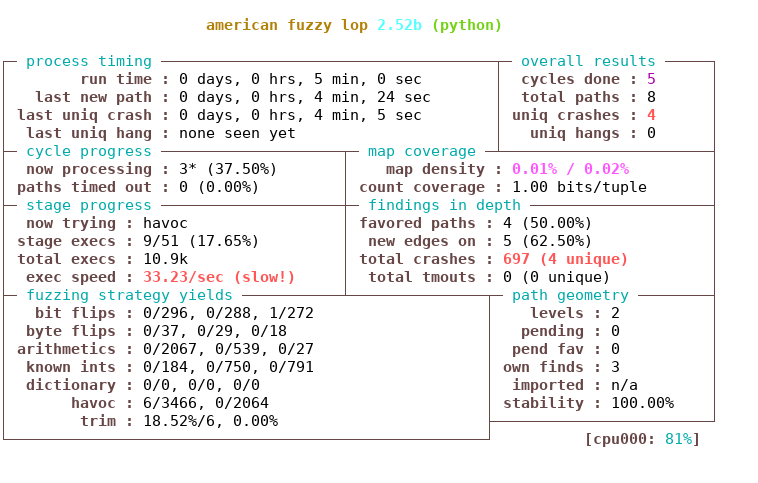
\includegraphics[scale=0.75]{images/afl-unicorn-sample.png}
  \caption{Run of afl-unicorn on the example template}
  \label{fig:aflunicornres}
\end{figure}

There are some other tools and fuzzers that can be used to test for more
vulnerabilities, for example some of the forks of \textbf{AFL} might produce better results and efficiently test these binaries. Other tools such as LLVM, which includes a fuzzer, a memory and an address sanitizer and Valgrind might be used to explore areas that \textbf{AFL} is not able to test.

\end{document}
